% Default course lecture note template by asp 
\documentclass[letterpaper]{article}
\usepackage[utf8]{inputenc}
\usepackage[T1]{fontenc}
\usepackage[english]{babel}
\usepackage[top=3cm, bottom=3cm, left=3.85cm, right=3.85cm]{geometry}
\usepackage[onehalfspacing]{setspace}
\usepackage{amsmath,amssymb,wasysym,amsthm}
\usepackage{graphicx}
\usepackage{mathptmx}
\usepackage{tikz}
\usepackage{float}
\usetikzlibrary{arrows, calc, positioning}
\usepackage{hyperref}
\usepackage{gitinfo}
\usepackage{xspace}
\usepackage{lineno}
\usepackage[tablename=Figure]{caption}
\title{Borromean~Ring~Signatures\footnote{This work was sponsored by Blockstream.}}
\author{
  Gregory Maxwell,
  Andrew Poelstra\footnote{
    \texttt{greg@xiph.org},
    \texttt{apoelstra@wpsoftware.net}}
}
\date{\gitAuthorDate{} (commit \texttt{\gitAbbrevHash)}}


% my usual newcommands
\newcommand{\pk}{\textnormal{\texttt{pk}}}
\newcommand{\sk}{\textnormal{\texttt{sk}}}

\begin{document}

\maketitle
\hyphenpenalty=15000
\pretolerance=10000
\interfootnotelinepenalty=10000

\begin{abstract}
In 2002, Abe, Ohkubo, and Suzuki developed a new type of ring signature based
on the discrete logarithm problem, which used a novel commitment structure to
gain significant savings in size and verification time for ring
signatures\cite{abe+ohkubo+suzuki2002}.

Ring signatures are signatures using $n$ verification keys which require
knowledge of one of the corresponding secret keys. They can therefore be
considered a signature of a disjunctive statement ``I know $x_1$ OR I know
$x_2$ OR \ldots''. We generalise their construction to handle conjunctive
statements ``I know one of $\{x_1, x_2, x_3, \ldots\}$ AND one of
$\{x_4, x_5, x_6, \ldots\}$ AND \ldots''
and thereby gain the ability to express knowledge of any monotone boolean
function of the signing keys.

This can be trivially done by use of multiple independent ring signatures;
our construction saves space relative to this by sharing commitments
across the individual rings.

We also describe a new way of thinking about these ring signatures, and
ordinary Schnorr signatures, in terms of ``causal loops'' which may provide
a framework for further generalisations.
\end{abstract}

\clearpage

\paragraph{License.} This work is released into the public domain.

\modulolinenumbers[10]
\linenumbers

\section{Random oracles and Schnorr signatures}

Throughout we assume we are working in a cyclic additive group $\mathcal{G}$ for
which the discrete logarithm problem is hard, and that $G$ is some fixed known
generator of the group.

\subsection{Schnorr authentication}
Consider the following interactive authentication protocol, developed by Claus
Schnorr in 1989\cite{schnorr1989}, which allows the possessor of a secret discrete
logarithm $x$ of a public group element $P=xG$ to prove knowledge of $x$ without
revealing anything about it:
\begin{enumerate}
\item The prover chooses a random scalar $k$ and submits $kG$ to the verifier.
\item The verifier responds with a random challenge scalar $e$.
\item The prover replies with the scalar $s\gets k + xe$.
\end{enumerate}
The verifier does not know $k$, since the discrete logarithm problem is hard,
but can check that $s$ was computed honestly because $s = k + xe$ is equivalent
to $sG = kG + exG$ and the verifier knows each of $s$, $e$, $kG$ and $xG$.

Intuitively, this is zero knowledge because if the verifier had slipped the
prover pre-knowledge of what $e$ would be, the prover could have produced a
legitimate $s$ without knowing $x$ at all. (Specifically, she would choose
$s$ randomly and then choose ``$kG$'' as $sG - exG$.) The transcript of the
prover/verifier interactions in this case would be statistically indistinguishable
from a transcript in the honest game; thus if the dishonest game revealed
nothing about $x$ (and it did not; it did not even use $x$!) then neither did
the honest one.

Intuitively, it proves that the prover knows $x$, since $e$ was chosen uniformly
at random. If she could win no matter what $e$ was, then it is a simple matter to
``fork'' her and give each fork different $e$ values, say $e_1$ and $e_2$. Then
the two forks would produce $s_1 = k + xe_1$ and $s_2 = k + xe_2$, which expose
$x$ as $x = (s_1 - s_2)/(e_1 - e_2)$. In other words, a verifier that can win
regardless of $e$ can be used to extract the value of $x$, and therefore she must
have knowledge of it.

\subsection{Random oracles and Fiat-Shamir}

The above scheme is not \emph{publicly verifiable}, for exactly the same reason
that it is zero-knowledge. That is, a transcript of the interaction between the
prover and verifier is indistinguishable from one in which they were colluding
to avoid anybody knowing $x$. Therefore, in the honest game, the prover proves
knowledge of $x$ to the verifier, but not to anybody else.

Fortunately, since the verifier has no purpose except to produce random values
in response to challenges, it has a very simple mathematical description: that
of a \emph{random function}. Random functions are mathematical functions which
return independent uniformly random values on each input. ``Evaluating''
such a function is functionally equivalent to submitting a challenge value
and receiving a new random value on each new input. Therefore random functions
are often referred to as \emph{random oracles}.

Random functions have infinite Kolmogorov complexity and cannot be instantiated
in a machine, but we replace them by simple functions called \emph{hash functions}
for which there is no known way to distinguish them from random.
This gives us the so-called \emph{random oracle model}\cite{bellare+rogaway1993},
in which we effectively have a challenger who exists in the world of Platonic
forms\cite{ross1951}, and whom we refer to as a random oracle.

Random oracles have two benefits over traditional challengers: (a) the oracle's
behaviour is publicly verifiable and can be seen not to be behaving dishonestly,
so by ``proving to the oracle'' knowledge of a discrete logarithm, one actually
proves this knowledge to everyone; (b) the oracle is modelled by a hash function
which can be computed by anyone to recreate the transcript of interaction, so
there is no need for any actual interaction.

The idea of replacing an actual challenger with a random oracle is known as the
\emph{Fiat-Shamir transform}\cite{fiat+shamir1986} after the first to use the idea to
turn an interactive scheme into a non-interactive publicly verifiable one.
Applying the Fiat-Shamir transform to the above interactive scheme gets us
the \emph{Schnorr signature scheme} which works as follows:
\begin{enumerate}
\item The prover chooses a random scalar $k$ and computes $e = H(kG)$.
\item The prover computes the scalar $s\gets k + xe$ and publishes $(s, e)$.
\end{enumerate}
Since $H$ returns a different $e$ for different inputs, it is possible to add
things to its input; for example, computing $H(m\|kG)$ for some message $m$.
The result is a transcript containing $m$ for which $m$ cannot be changed
without knowledge of $x$. This is thus a ``signature of knowledge'' on $m$.

Anyone can verify the signature's veracity by first computing $kG = sG - eP$
and checking that this is actually the committed value; \emph{i.e.}, that
$e\stackrel{?}{=}H(kG)$.
The fact that $P=xG$ is used in the verification is what ties this signature
to $x$.

\section{Ring signatures}

\subsection{Time travel and chameleon hashes}

The critical ingredient of the above authentication scheme is the \emph{time
ordering}. We observed that if the prover could see into the future and
determine $e$ before choosing $kG$, she could successfully authenticate
without knowing $x$.

In the random oracle model, there is no more interaction and therefore no
more time. However, the random oracle $H$ provides its own time ordering:
since for any input $y$ it is impossible to know $H(y)$ without evaluating
it (except by guessing it, which succeeds with only negligible probability),
we can say that $H(y)$ is determined ``after'' $y$. We therefore preserve
the idea of time being essential, though our definition of time has changed.

This definition of time admits a cryptographic trick to allow the possessor
of some secret knowledge to reverse it. The way this works is to tweak our
hash function $H$ to make it a \emph{chameleon hash}\cite{krawczyk+rabin1997}. A chameleon hash,
rather than taking just an input $e$, also takes as input a random value $s$.
A possessor of some secret ``trapdoor'' information
will be able to tweak $s$ so as to change $e$ without changing the hash output,
while ordinary mortals remain bound by the laws of time: once the hash of
$e$ is computed, $e$ is in the past and cannot be changed any more than
you can choose not to have read this sentence.

We define a chameleon hash from an ordinary hash $H$ as follows. Here
$G$ and $P$ are generators of the group; the trapdoor information is
$x$ such that $P = xG$. Our hash function is
\[ H'(m, e, s) = H(m\|sG - eP) \]
(This is actually a ``half-chameleon hash'': someone with trapdoor information
can change the value of $e$ by changing $s$ appropriately\footnote{Specifically,
if $h = H'(m, e, s)$, then to change $e$ to $e'$ one sets $s'\gets s +
(e - e')x$, so $s'G - e'P = sG - eP$ and thus $H'(m, e', s') = H(m,e,s)$.},
but nobody can change $m$ without changing the output of the hash function.)

We notice that if $s = k + xe$, which is the value $s$ from a Schnorr signature,
then $e = H'(m, e, s) = H(m\|kG)$ can be computed without foreknowledge of $e$.
We can therefore describe Schnorr signatures as a pair $(s, e)$ where $e$ is
both the input and output of a chameleon hash and $s$ is its random input.
Since the output of the hash is random and independent of its input, forcing
the input to be equal to the output requires trapdoor information, and is thus a
proof that the signer has this information.
The result is called a \emph{signature of knowledge}.

In other words,
we can think of Schnorr signatures as working as follows: to produce a
Schnorr signature without knowing the secret key $x$, one must predict
the output of random oracle $H$, effectively ``travelling backward in time''.
The signature is structured to essentially contain a hash of itself,
creating a causal loop and forcing signers to know the trapdoor information.

In the next section we will generalise these causal loops and see that
they are a useful abstraction.

\subsection{Abe-Ohkubo-Suzuki ring signatures}

\emph{Ring signatures} are a variant of digital signatures in which the
verification key is replaced by a set, or \emph{ring}, of verification keys.
Each verification key has a corresponding secret key, and only one is
required to produce a ring signature. However, all of the verification keys
play the same role in verifying the signature, so the specific signing key
used remains secret.

Ring signatures were introduced by Rivest, Shamir, and Tauman\cite{rivest+shamir+tauman2001}
in 2001. Their suggested use-case was whistleblowing: a well-connected signer
could construct a ring with the verification keys of other well-connected
parties, then sign a message blowing the lid off some conspiracy. Verifiers
would see that somebody well-connected had signed off on the leak, giving it
veracity, but they would not know who specifically had done it, preventing
nasty personal consequences.

In 2002, Abe, Ohkubo, and Suzuki developed a new type of ring signature based
on the discrete logarithm problem\cite{abe+ohkubo+suzuki2002}, which used
causal loops (though they did not use the term) to obtain the ring property.
This use of causal loops gave a significant (50\%) reduction in the size of
the signatures compared to earlier ring signatures. It is described as follows.

\begin{figure}\label{fig1}
\begin{center}
\begin{tikzpicture}[->,>=stealth',shorten >=1pt]
  %% schnorr
  \node[draw, circle] (A1) {$e$};
  \path
    (A1) edge [dashed, loop right, color=red] node[color=black] {(s, P)} (e);

  %% 2-coin steal
  \node[draw, circle, right = 2in of A1] (B2) {$e_1$};
  \node[draw, circle, above = 1in of B2] (A2) {$e_2$};
  \node[draw, circle, below = 1in of B2] (C2) {$e_0$};

  \path
    (A2) edge node[left] {$(s_2, P_2)$} (B2)
    (B2) edge node[left] {$(s_1, P_1)$} (C2)
    (C2) edge[dashed, bend right, color=red] node[right, color=black] {$(s_0, P_0)$} (A2);

  \node[below=0.5in of C2] (T1) {AOS Signatures (1 of 3)};
  \node[left=1in of T1] (T2) {Schnorr Signature (1 of 1)};
\end{tikzpicture}
\end{center}
\caption{Schnorr as a special-cased AOS signature}
\end{figure}

In this scheme, rather than having $kG = sG - exG$ committed to by $e$, we
have a set of hashes $\{e_i\}_{i=0}^{n-1}$, each committing to $k_iG = s_iG
- e_iP_i$, where the indices are considered modulo $n$. Since each $e_i$ commits
to the $s_{i-1}$ before it, it is easy to produce values for $k_iG$ --- just
choose $s_i$ at random and compute the resulting $k_iG$ and $e_i$! The signer can
do this starting with any index $j$: first compute $e_j$ as the hash of some
random $k_jG$, then using this compute $(s_{j+1}, e_{j+1})$, then $(s_{j+2}, e_{j+2})$,
and so on until reaching $(s_j, e_j)$.

However, when computing $(s_j, e_j)$, the signer finds that $e_j$ has already
been determined (this was the first step). He must somehow compute $s_j$
to fit. Just like with the ordinary Schnorr signature, to do this requires ``going
back in time'' to choose an $s_j$ value compatible with $e_j$, and just
like with the ordinary Schnorr signature, this can be done as long as the signer
knows the discrete logarithm $x_j$ of $P_j$: set $s_j = k_j - x_je_j$. The
final signature is $\sigma = \{ e_0, s_0, s_1, \ldots, s_{n-1} \}$.

Since $s_j$ contains the random value $k_j$, it appears uniformly random, just
like every other $s_i$, and from the perspective of the verifier, there is nothing
special about the index $j$. The result is a signature which requires many verification
keys to verify, only one of whose secret key is required to produce. This is a ring
signature!

This has been very algebraic. We can extract the structure of the commitments to
see what is ``really'' going on with these ring signatures. We do this by drawing
them as directed graphs. The vertices of the graph are labelled by the chameleon
hash output; the incoming edges by their blinded input. (As in the Schnorr case,
the blinding either forces the value of the edge's source vertex or requires
some secret knowledge; the difference is that in the Schnorr case there is only
one edge whose source and target vertices are the same.)

In other words: as before, we have a
notion of time which mandates nothing more than that a hash $e$ can only be known
\emph{after} its input is decided. And as before, we can use chameleon hashes to
override this time-ordering (only) for people in possession of trapdoor information.
We can draw this time-ordering as a directed graph, and make two observations:
\begin{enumerate}
\item To form a cycle, it is necessary and sufficient to ``go back in time'' for
one commitment; that is, only one secret key is required.
\item From the perspective of a verifier, a reversed-time commitment is
indistinguishable from an ordinary one. Further, he can only see the graph
structure: the colouring and up/down distinction we have used in our illustrations
is invisible.
\end{enumerate}
These two observations together describe how the Abe-Ohkubo-Suzuki ring signature
works: it is simply a cycle of chameleon-hash commitments\footnote{As before,
we use half-chameleon hashes; each $e_i$ commits to the previous $e_{i-1}$
in a time-reversible way but commits to the message and verification key set
in an irreversible way, since these should not be tamperable.}.

\section{Borromean ring signatures}

With this background in place, the concept of Borromean ring signatures can be
described as a straightforward generalisation. Where ordinary ring signatures
take a set of verification keys $\{v_i\}_{i=1}^n$ and describe a signature
signed with $s_1$ OR $s_2$ OR $\cdots$ OR $s_n$, where $s_i$ is the secret
key corresponding to $v_i$, Borromean ring signatures can describe signatures
signed with arbitrary functions of the signing keys.

More formally,
let $\mathcal{V}$ be some set of verification keys, and $f$ be a function which
maps finite subsets of $\mathcal{V}$ to $\{0,1\}$. We call $f$ an \emph{admissibility
function}; then an \emph{admissible set} $V$ of verification keys is one for which
$f(V) = 1$.

A Borromean ring signature $\sigma$ is a signature on a message $m$ with a set
$\mathcal{V}$ of verification keys and admissibility function $f$ which
satisfy the following:
\begin{enumerate}
\item $\sigma$ can be produced only by parties who together know all the secret
keys to an admissible set $V$ of verification keys.
\item Given only $\sigma$, $\mathcal{V}$, and $m$, it is statistically
indistinguishable which admissible set $V$ was used.
\end{enumerate}

\subsection{Monotone functions}

We observe that if $V$ is an admissible set, without loss we may also assume
that any superset $V'$ is also admissible. The reason is that if $V$ is
admissible, then parties holding the signing keys to $V'$ are able to produce
valid signatures by simply ignoring the keys in $V'$ that are not in $V$.
We can therefore put the following restriction on $f$: if $f(V) = 1$, then
for all $V'\supseteq V$, $f(V') = 1$. Functions which satisfy this restriction
are called \emph{monotone functions}.

\subsection{AND and OR}

It can be shown\cite{benaloh+leichter1988} that monotone functions are exactly
those that can be represented by circuits in disjunctive normal form which have
no negations; \emph{i.e.}, circuits of the form
\[ \bigwedge_i \left(\bigvee_j a_{i,j}\right) \]
where $\bigwedge$ or AND outputs 1 iff all its inputs are 1; $\bigvee$ or OR
outputs 0 iff all its inputs are 0.

We observe that Abe-Ohkubo-Suzuki signatures can be described as Borromean ring signatures
whose admissibility function $f$ consists of a single OR gate. We observe more
generally that we can construct OR gates out of cycles, as described in an
earlier section.

To take the conjunction of these OR gates, it is sufficient to simply create
disjoint graphs, which would each correspond to a single AOS signature. However,
we can do better than this by creating a new graph structure corresponding to
the AND gate. Specifically, if we create a vertex $e$ with multiple outgoing edges
(meaning multiple $s$ values which individually either require secret knowledge
or force the value of $e$), then we have constructed an AND without requiring
multiple graphs.

It is easy to see how a signature can be structured so that its graph has
vertices with multiple outgoing edges: each edge $i$ from a vertex labelled
$(e,x)$ is labelled by a $s_i$ value which is either random (for forward-time
edges) or equal to $s_i = k_i - xe$ (for backward-time edges). However, to
force backward-time edges, we need to have every path be part of a cycle. This
forces us to also have vertices with multiple \emph{incoming} edges (see vertex
$e_0$ in Figure \ref{fig2}). This means we need to change our commitment structure.

Recall that for a vertex $(e,\cdot)$ with a single incoming edge $s$ (whose source
vertex is $(e',x')$), the value $e$ is computed by chameleon hash as
\[ e = H(m\| sG - e'x'G) \]
If we have multiple incoming edges $\{s_i\}_{i=1}^n$ whose source vertices are
$\{(e_i,x_i)\}_{i=1}^n$, the generalisation is obvious:
\[ e = H(m\| s_1G - e_1x_1G \| \cdots \| s_nG - e_nx_nG) \]
The result is a ``multiply-chameleon hash'': each $x_i$ is a piece of trapdoor
information which can be used independently to make its corresponding edge $s_i$
go backward in time. This is exactly the structure we would expect from a vertex
in our graph with multiple incoming arrows.
\clearpage

With these pieces in place, we are able to draw a graph describing a Borromean
signature:
\begin{figure}[H]
\begin{center}
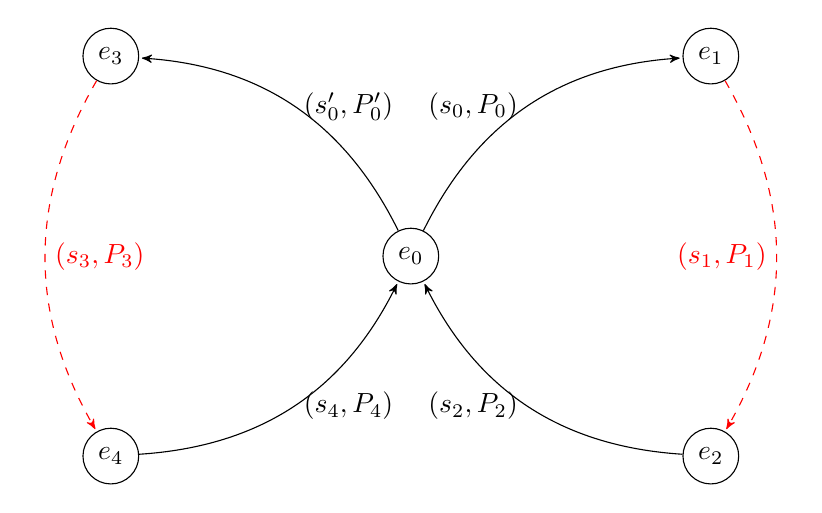
\begin{tikzpicture}[->,>=stealth',shorten >=1pt]
  \node[draw, circle] (e0) at (0in, 0in)     {$e_0$};
  \node[draw, circle] (e1) at (1.5in, 1in)   {$e_1$};
  \node[draw, circle] (e2) at (1.5in, -1in)  {$e_2$};
  \node[draw, circle] (e3) at (-1.5in, 1in)  {$e_3$};
  \node[draw, circle] (e4) at (-1.5in, -1in) {$e_4$};

  % left circle
  \path
    (e0) edge[bend right] node[right] {$(s_0', P_0')$} (e3)
    (e3) edge[bend right, dashed, color=red] node[right] {$(s_3, P_3)$} (e4)
    (e4) edge[bend right] node[right] {$(s_4, P_4)$} (e0);
  % right circle
  \path
    (e0) edge[bend left] node[left] {$(s_0, P_0)$} (e1)
    (e1) edge[bend left, dashed, color=red] node[left] {$(s_1, P_1)$} (e2)
    (e2) edge[bend left] node[left] {$(s_2, P_2)$} (e0);
\end{tikzpicture}
\end{center}
\caption{A Borromean ring signature for $(P_0 | P_1 | P_2) \& (P_0' | P_3 | P_4)$\label{fig2}}
\end{figure}

Though it would result in a more crowded picture, it is clear how this scales
to more than two rings; the resulting signature is one that can only be created
by knowing the discrete logarithms of one of $\{P_0, P_1, P_2\}$ \emph{and}
$\{P_0', P_3, P_4\}$, and we saved one commitment versus having separate rings.

In general, if we take the conjunction of $n$ rings, we save $(n-1)$ commitments
versus using separate ring signatures.

\subsection{Concrete algorithm}

The above has given a description of Borromean ring signatures in terms of graph
structures, and technically has all the information required to implement them.
However, the devil is in the details, and it is not obvious that it is
actually possible to compute these signatures. We therefore lay out the actual
signing and verification algorithms.

\subsubsection{Signing}

Suppose a signer has a collection of verification keys $P_{i,j}$ for
$0\leq i\leq n-1$, $0\leq j\leq m_i-1$, and wants to create a signature
of knowledge of the $n$ keys $\{P_{i,j^*_i}\}_{i=0}^{n-1}$ where the
$j^*_i$'s are some fixed and unknown (to a verifier) indices. Denote the
secret key to $P_{i,j^*_i}$ by $x_i$. He acts as follows:

\begin{enumerate}
\item Compute $M$ as the hash of the message to be signed and the set of
verification keys.
\item For each $0\leq i\leq n-1$:
\begin{enumerate}
\item Choose a scalar $k_i$ uniformly at random.
\item Set $e_{i,j^*_i+1} = H(M\| k_iG \| i \| j^*_i)$.
\item For $j$ such that $j^*_i+1\leq j< m_i-1$ choose $s_{i,j}$ at random and
compute
\[ e_{i,j+1} = H(M\| s_{i,j}G - e_{i,j}P_{i,j} \| i \| j). \]
\label{comp1}
\end{enumerate}
\item Choose $s_{i,n_j}$ for each $i$ at random and set
\[ e_0 = H(s_{0,m_0-1}G - e_{0,m_0-1}P_{0,0} \| \cdots \| s_{n-1,m_n-1}G - e_{n-1,m_n-1}P_{n-1,m_{n-1}-1}) \]
That is, $e_0$ commits to several $s$-values, one from each ring.
\item For each $0\leq i\leq n-1$:
\begin{enumerate}
\item For $j$ such that $0\leq j< j^*_i$ choose $s_{i,j}$ at random and
compute
\[ e_{i,j+1} = H(M\| s_{i,j}G - e_{i,j}P_{i,j}\|i\|j). \]
where ``$e_{i,0}$'' means $e_0$. Note that this calculation is identical to
the one in Step $\ref{comp1}$.
\item Set $s_{i,j^*_i} = k_i + x_ie_{i,j^*_i}$.
\end{enumerate}
\end{enumerate}

The resulting signature on $m$ consists of
\[ \sigma = \{ e_0, s_{i, j} : 0\leq i\leq n-1, 0\leq j\leq m_i - 1 \} \]

\subsubsection{Verification}

Since verification does not depend on which specific keys are known, it
avoids the ``two-phase'' structure of signing and is therefore much
simpler.

We assume we have a message $m$, a collection $\{ P_{i,j} \}$ of verification
keys whose indices range as before, and a signature $\sigma$ whose notation
is the same as before. The verifier acts as follows:

\begin{enumerate}
\item Compute $M$ as the hash of the message to be signed and the set of
verification keys.
\item For each $0\leq i\leq n -1$,
      for each $0\leq j\leq m_i - 1$, compute $R_{i,j+1} = s_{i,j}G + e_{i,j}P_{i,j}$
and $e_{i,j+1} = H(M\|R_{i,j+1}\|i\|j+1)$. (As before, we always take $e_{i,0}$ to be $e_0$.)
\item Compute $e_0' = H(R_{0,m_0-1} \|\cdots \| R_{n-1,m_{n-1}-1})$ and return 1 iff $e_0'\stackrel{?}{=} e_0$.
\end{enumerate}

\subsection{Efficiency comparison}

Finally, we compare our scheme to existing ring signatures. We consider signing
with $N$ verification keys across $n$ rings.

\begin{center}
\begin{tabular}{|l|c|}
\hline
\textbf{Scheme} & \textbf{Size of signature}	\\
\hline
\parbox[t]{6cm}{$n$ original CDS ring signatures\cite{cramer+damgard+schoenmakers1994}\\
(for example, used by Monero)} & $2N$	\\
\hline
$n$ AOS ring signatures & $N + n$	\\
\hline
1 Borromean ring signature & $N + 1$	\\
\hline
\end{tabular}
\end{center}
Here ``size'' is measured in field elements or hashes, which are 32 bytes for
128-bit security.

\section{Open Problems}

In the above, we developed signatures which are proportionate in size to the
number of $a_{i,j}$'s in the disjunctive normal form expression.
\[ \bigwedge_i \left(\bigvee_j a_{i,j}\right) \]
By avoiding disjunctive normal form it is possible to represent these circuits
in much less space; however, it is unclear how the signatures corresponding
to such circuits should be structured.

Similarly, by using threshold gates rather than only AND and OR, a space
savings can be obtained for many monotone functions; it is also open how to
translate this to our framework.


\nolinenumbers
\clearpage
\bibliographystyle{amsalpha}
\bibliography{asp}

\end{document}

